\documentclass[11pt, oneside]{article}
\usepackage[letterpaper, margin=2cm]{geometry}
\usepackage{AERE546}
\usepackage{xspace}
\newcommand{\xb}{\bar{x}}
\newcommand{\yb}{\bar{y}}

\begin{document}
\noindent \textbf{\Large{Caleb Logemann \\
AER E 546 Fluid Mechanics and Heat Transfer I \\
Homework 8
}}

%\lstinputlisting[language=MATLAB]{H01_23.m}
\begin{enumerate}
  \item % #1
    The following is my code for the linear combination of upwinding and downwinding.
    \lstinputlisting[language=MATLAB]{upwindDownwind.m}

    \begin{enumerate}
      \item[\#1a]
        The plot for $p = 0.5$ and $c = 0.3$ is shown below.
        Initially the solution is represented well, but eventually the solution diverges.
        \begin{center}
          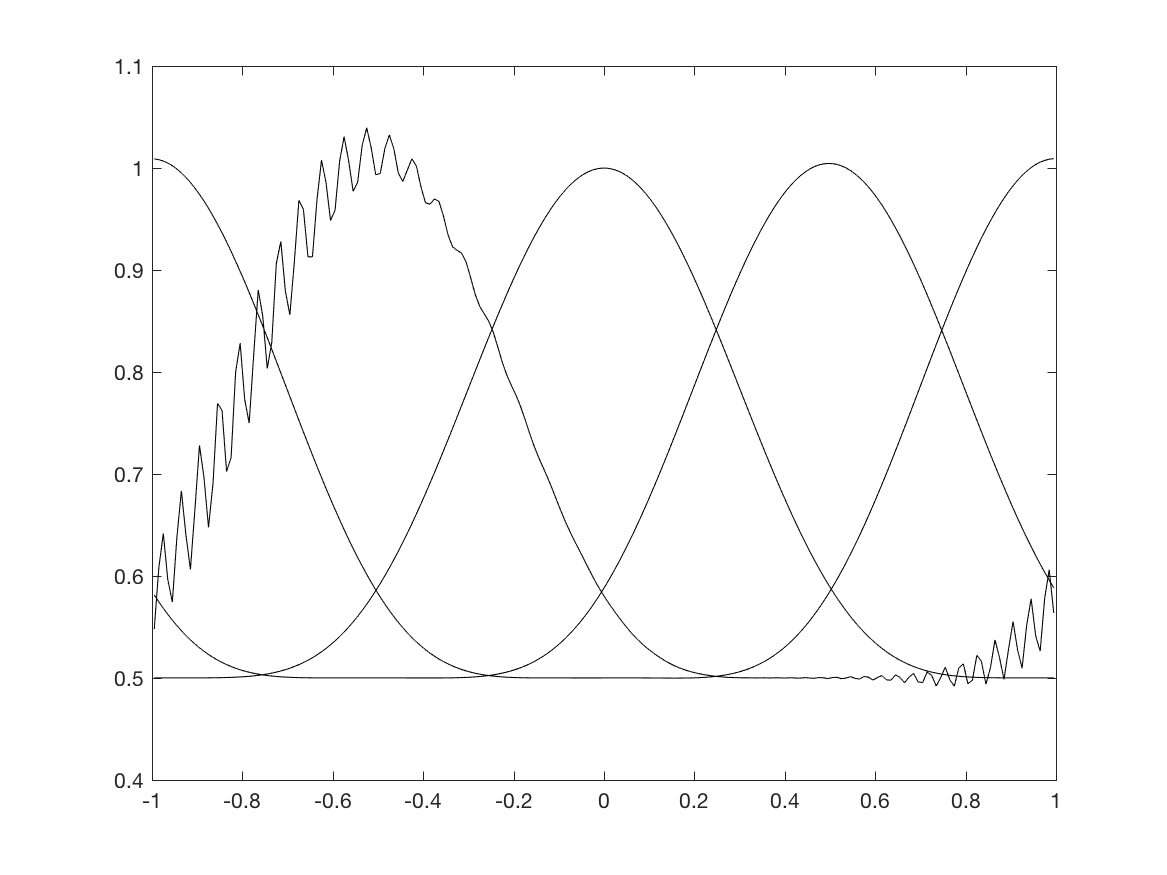
\includegraphics[scale=0.5]{Figures/08_01.png}
          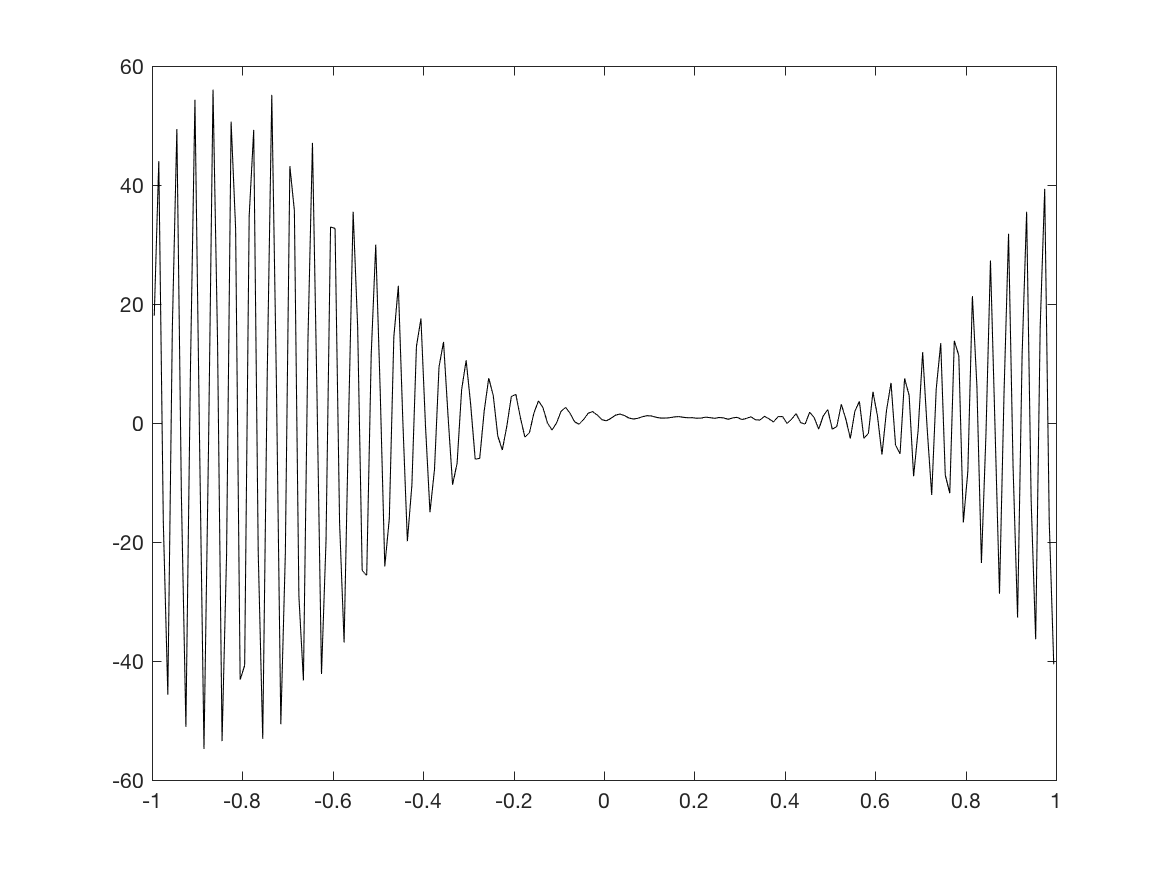
\includegraphics[scale=0.5]{Figures/08_02.png}
        \end{center}

      \item[\#1b]
        The solution diverges because with $p = 0.5$ this is identical to the
        central differencing scheme, which we know to be unstable for all cfl
        conditions.

      \item[\#2a]
        For $p = 1.0$ we have complete upwinding and the solution plots are
        \begin{center}
          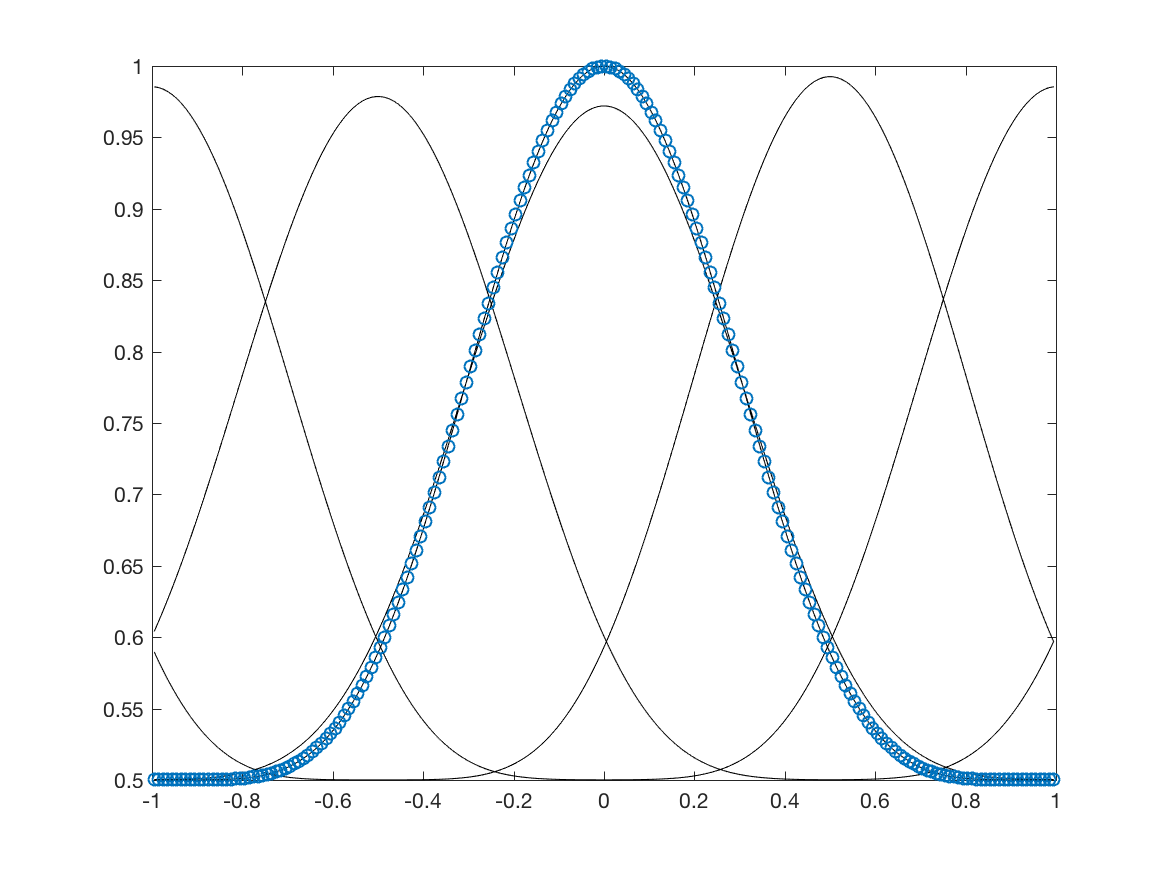
\includegraphics[scale=0.5]{Figures/08_03.png}
        \end{center}

      \item[\#2b]
        The simulated solution and the exact solution at $t = 2.0$ differ
        because upwinding is diffusive, so the numerical solution has
        decayed/diffused some instead of just convecting.

      \item[\#3a]
        For $p = 0.55$ and $c = 0.1$ the following plot is produced.
        \begin{center}
          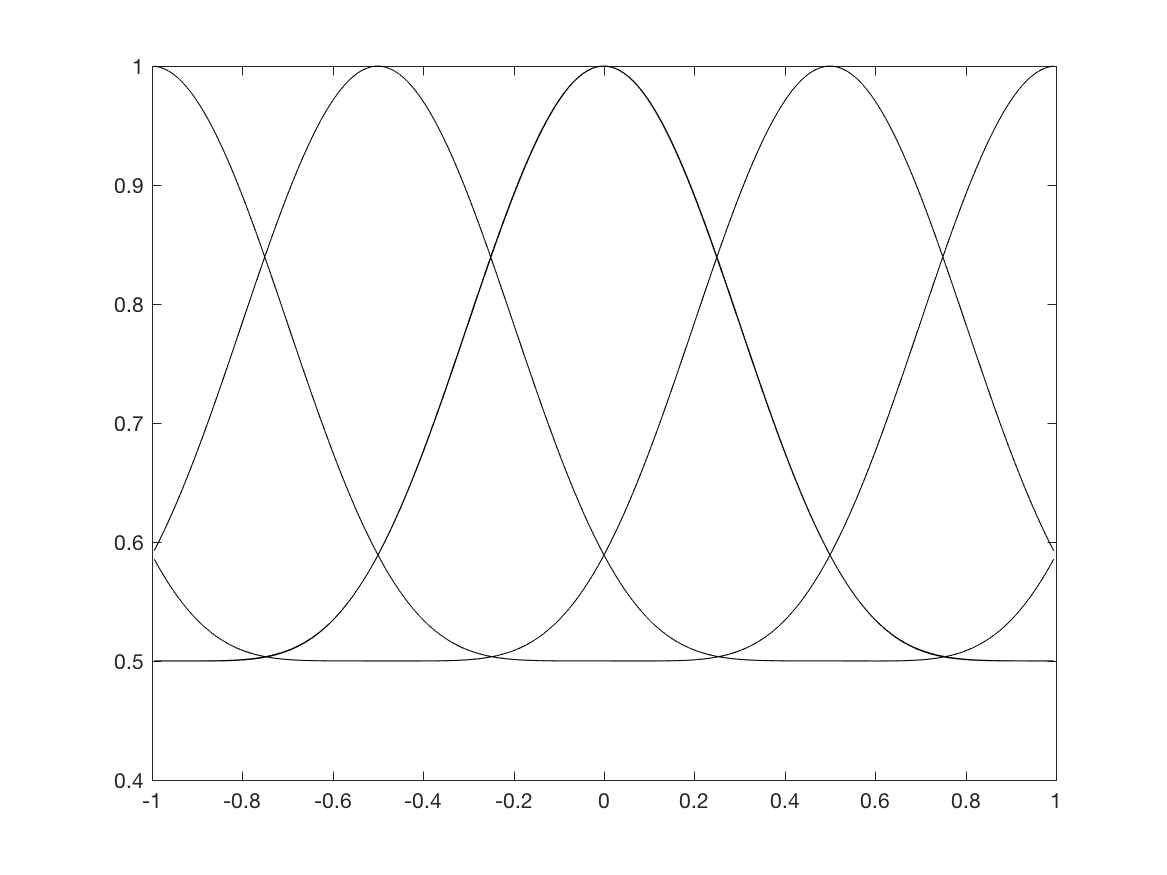
\includegraphics[scale=0.5]{Figures/08_04.png}
        \end{center}

      \item[\#3b]
        I found that the solution was accurate at $t = 2.0$ up to $c = 0.33$.

      \item[\#4]
    \end{enumerate}

  \item % #2

    The following two functions evaluate the RHS for the central and
    upwinding discretizations.
    These functions are used with the RK2 function that we have been using.
    \lstinputlisting[language=MATLAB]{central.m}
    \lstinputlisting[language=MATLAB]{upwind.m}
    These next two function run the Lax-Wendroff and MacCormack methods.
    \lstinputlisting[language=MATLAB]{laxWendroff.m}
    \lstinputlisting[language=MATLAB]{maccormack.m}

    The following images are produced.
    Note that the central differencing is unstable, but the lower cfl
    improves this.
    The upwind method is stable and doesn't produce any oscillations.
    However the second order methods, MacCormack and Lax-Wendroff do produce
    oscillations after the shock occurs.
    \begin{center}
      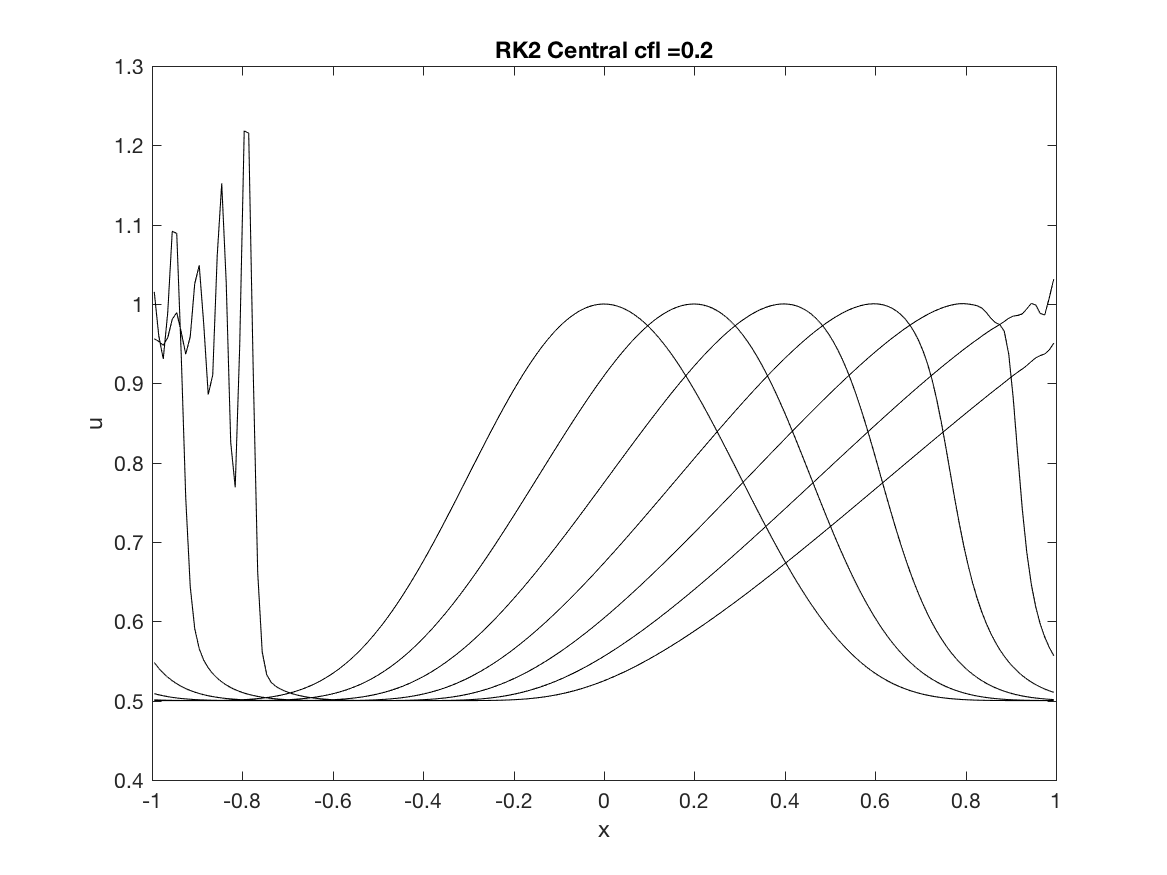
\includegraphics[scale=0.5]{Figures/08_05.png}
      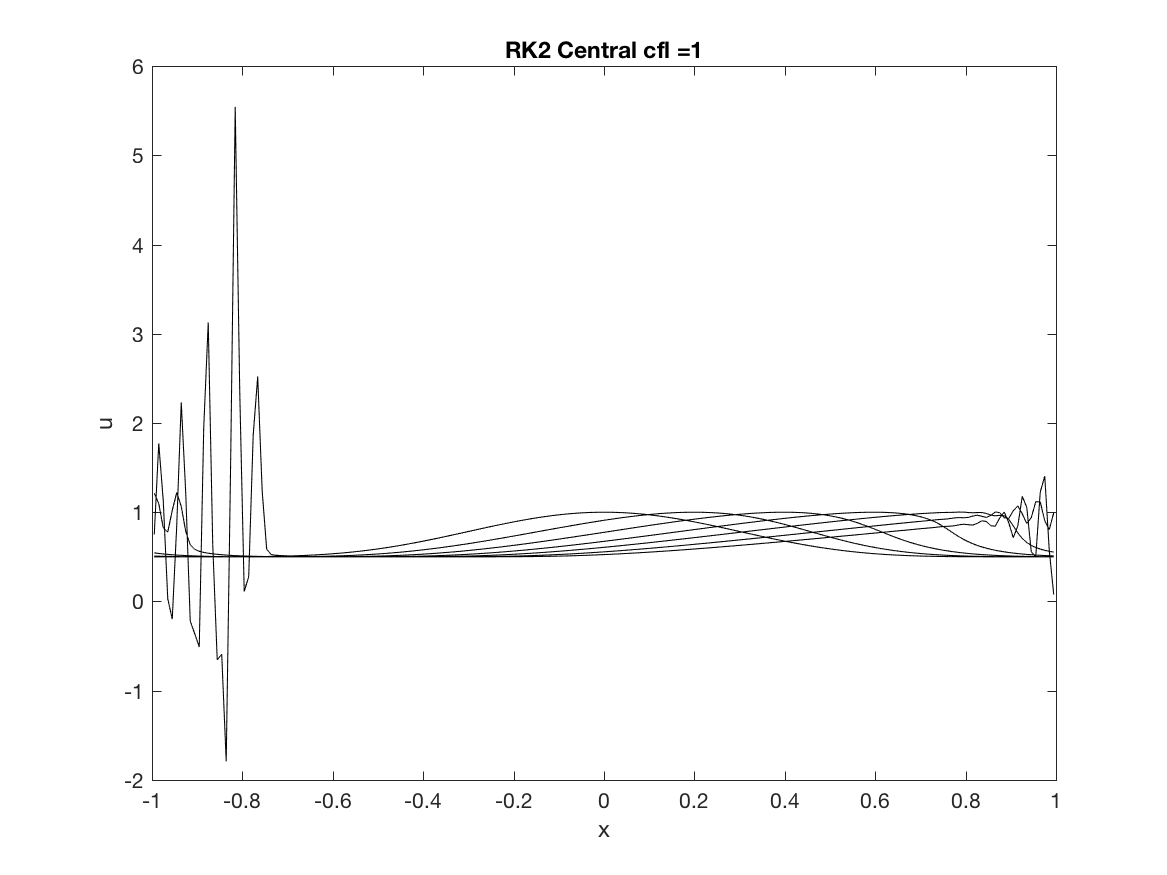
\includegraphics[scale=0.5]{Figures/08_06.png}
      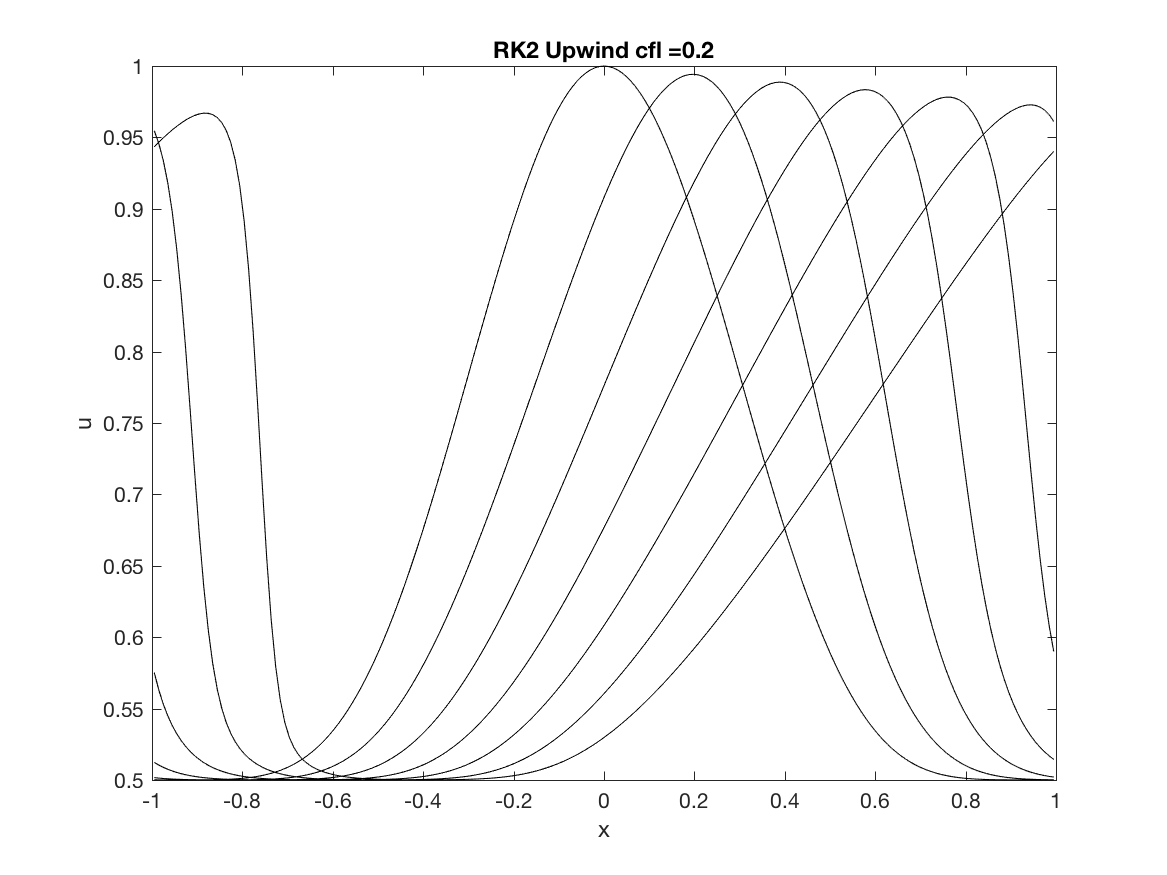
\includegraphics[scale=0.5]{Figures/08_07.png}
      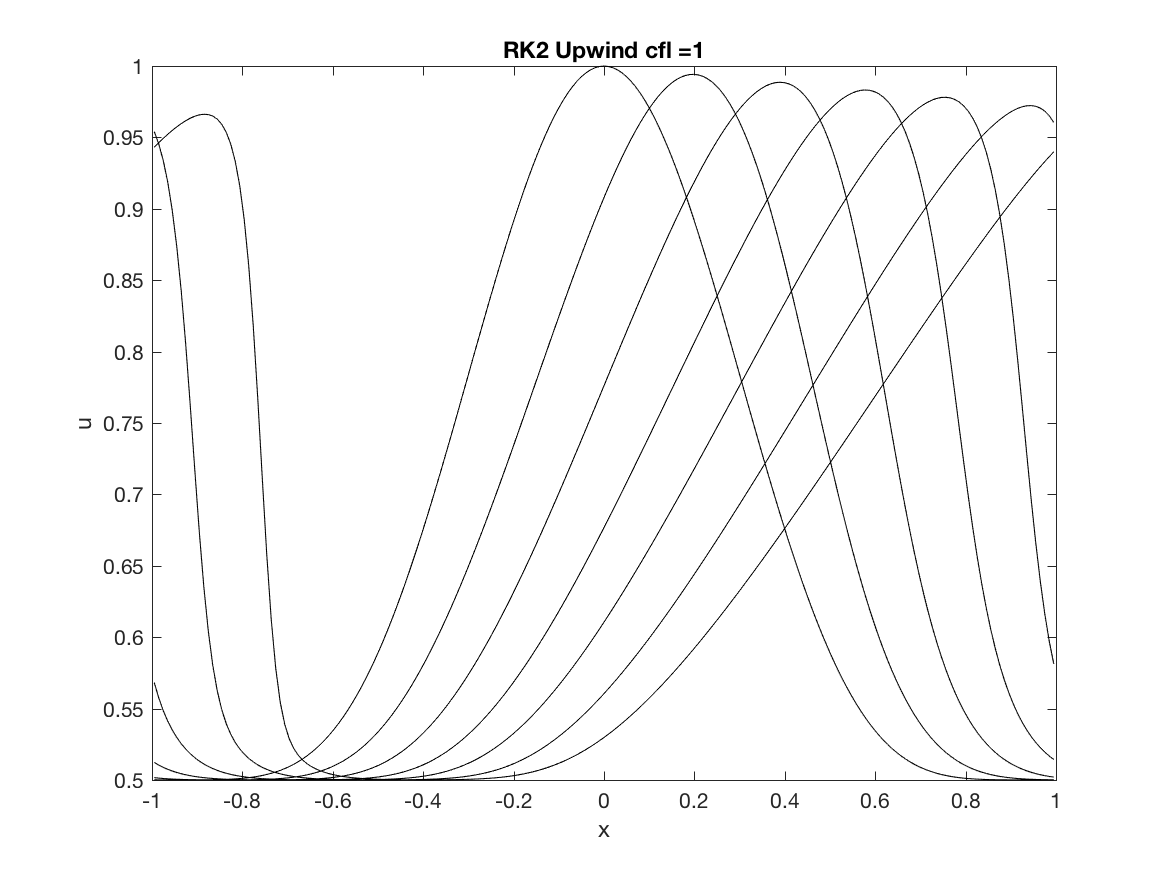
\includegraphics[scale=0.5]{Figures/08_08.png}
      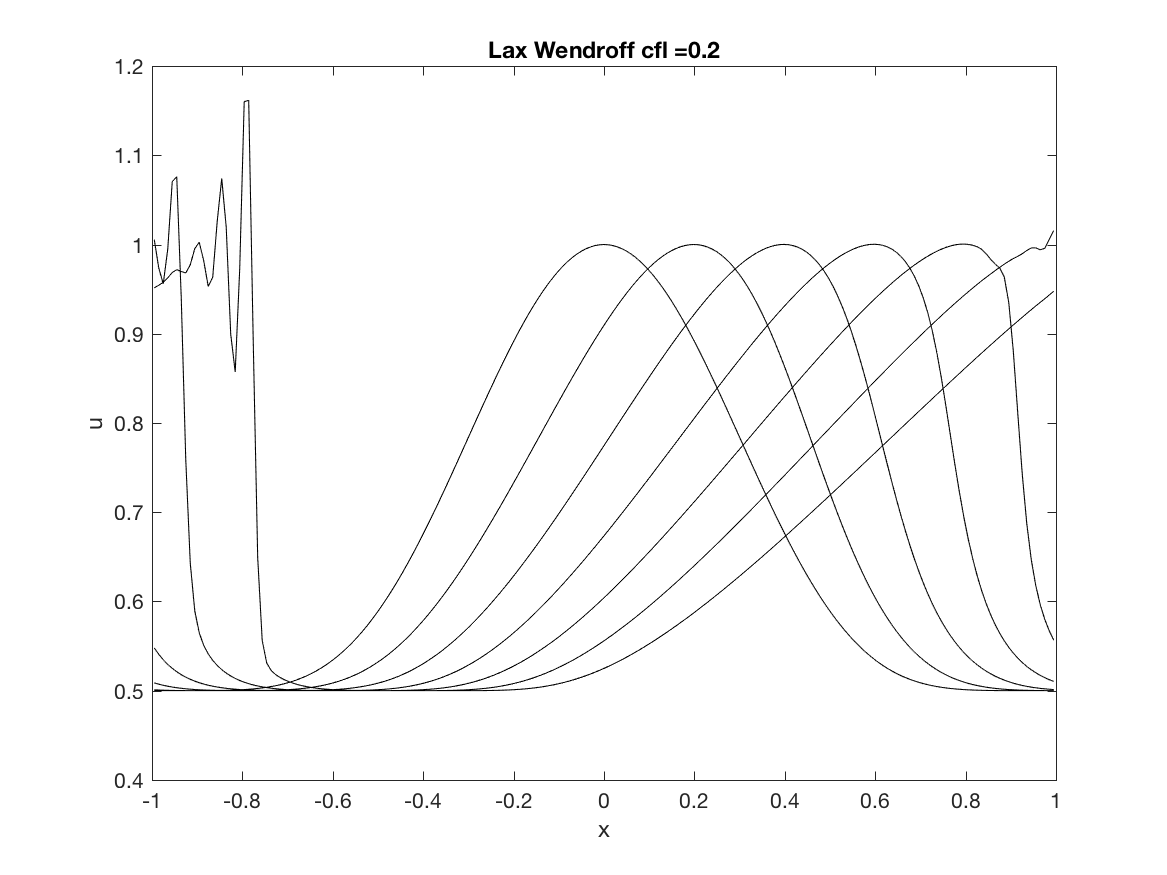
\includegraphics[scale=0.5]{Figures/08_09.png}
      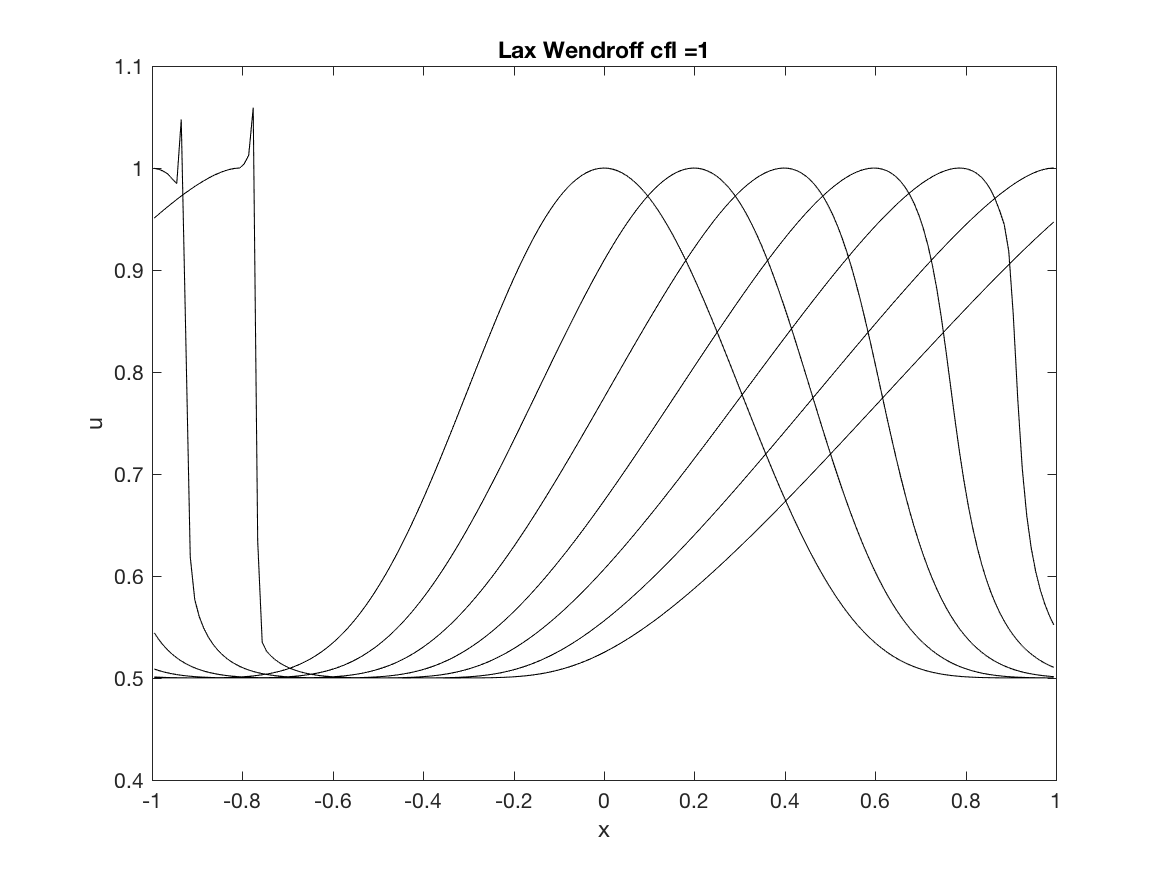
\includegraphics[scale=0.5]{Figures/08_010.png}
      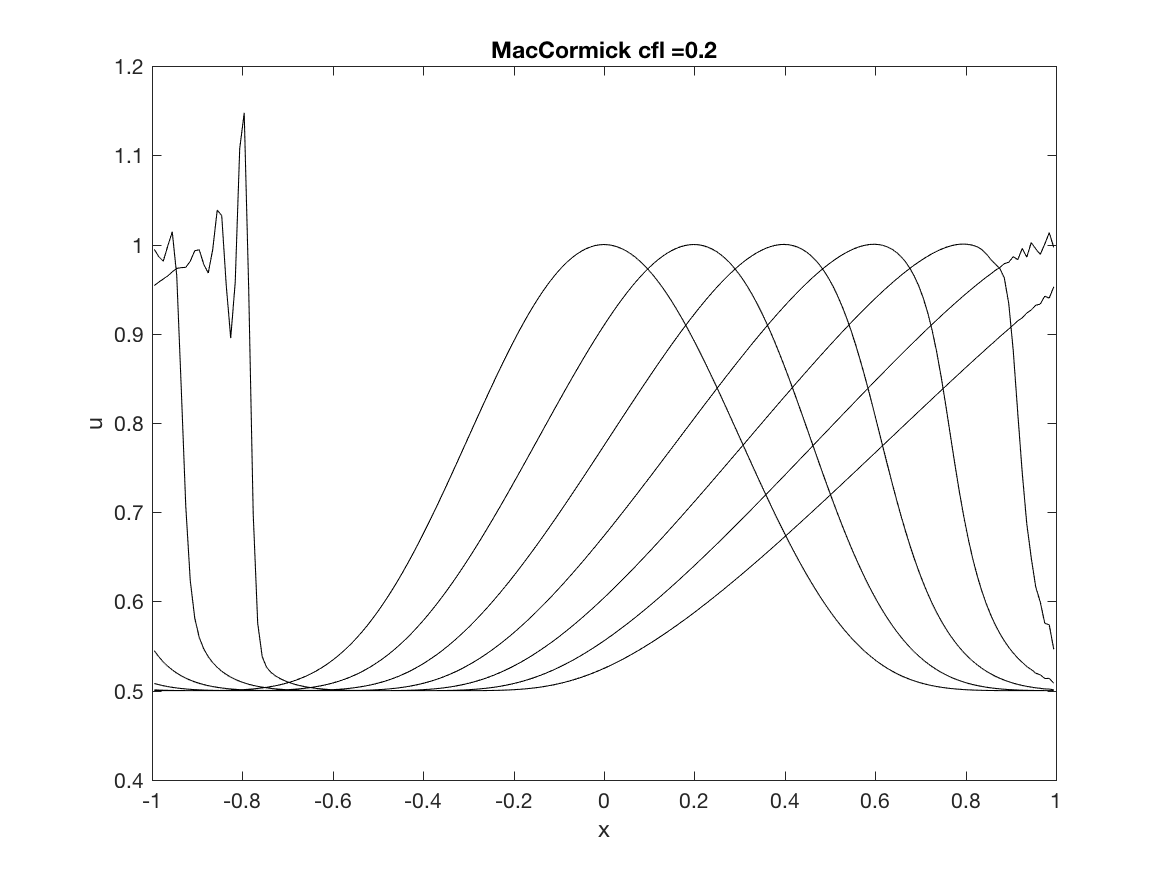
\includegraphics[scale=0.5]{Figures/08_11.png}
      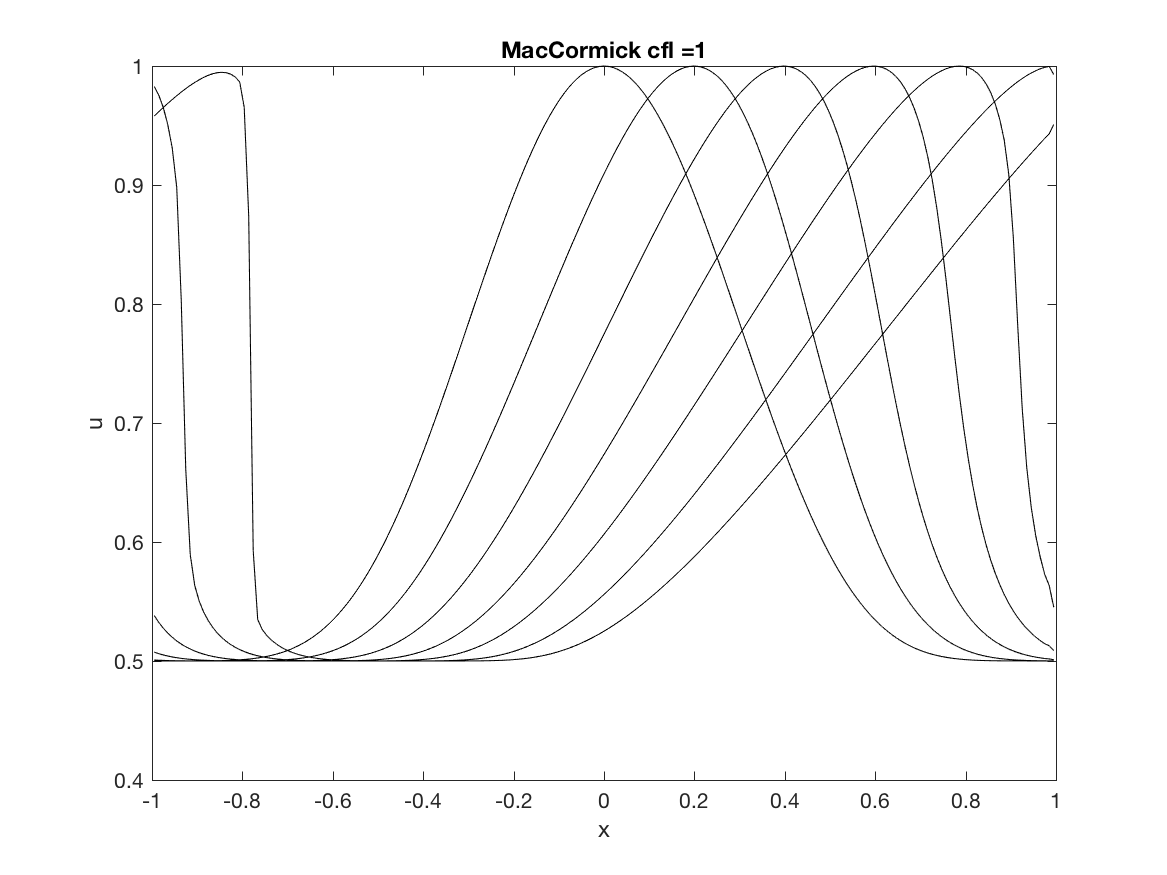
\includegraphics[scale=0.5]{Figures/08_12.png}
    \end{center}

  \item % #3
    I used the same RK2 upwind in conservation form and Lax-Wendroff method as
    shown in problem 2.
    However for RK2 in convection form the following is my RHS function.
    \lstinputlisting[language=MATLAB]{upwindConvection.m}

    For Burger's equation the shock speed is the average of the upper and lower
    states, so for this problem the shock velocity will be 1/2.

    The following images are produced.
    The RK2 method with upwinding in conservation form is stable and the
    shock moves at the correct speed.
    The diffusion of the full height of the wave can be seen.
    \begin{center}
      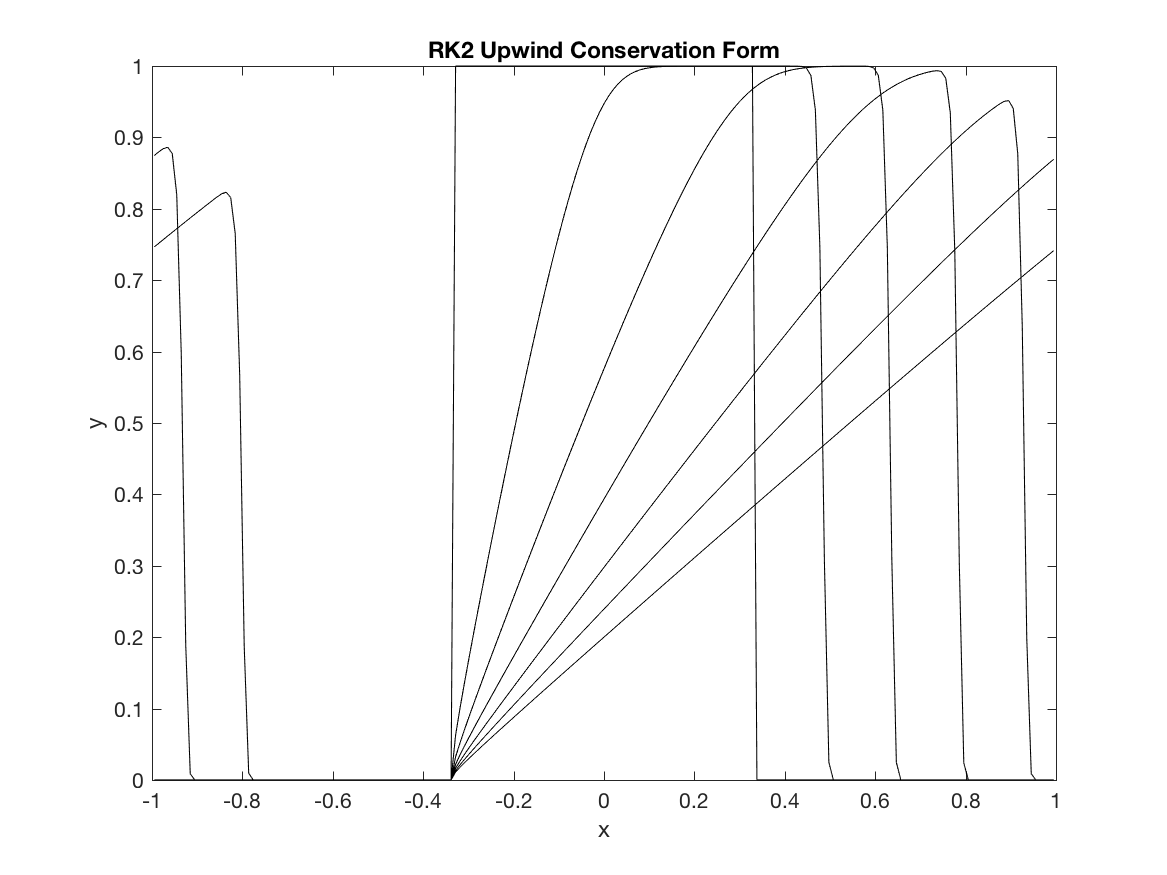
\includegraphics[scale=0.5]{Figures/08_13.png}
    \end{center}

    For the RK2 method with upwinding in convection form the shock does
    not travel at the correct velocity.
    In fact the shock doesn't travel at all.
    This method is stable and doesn't blow up, but it doesn't converge to the
    correct solution.
    \begin{center}
      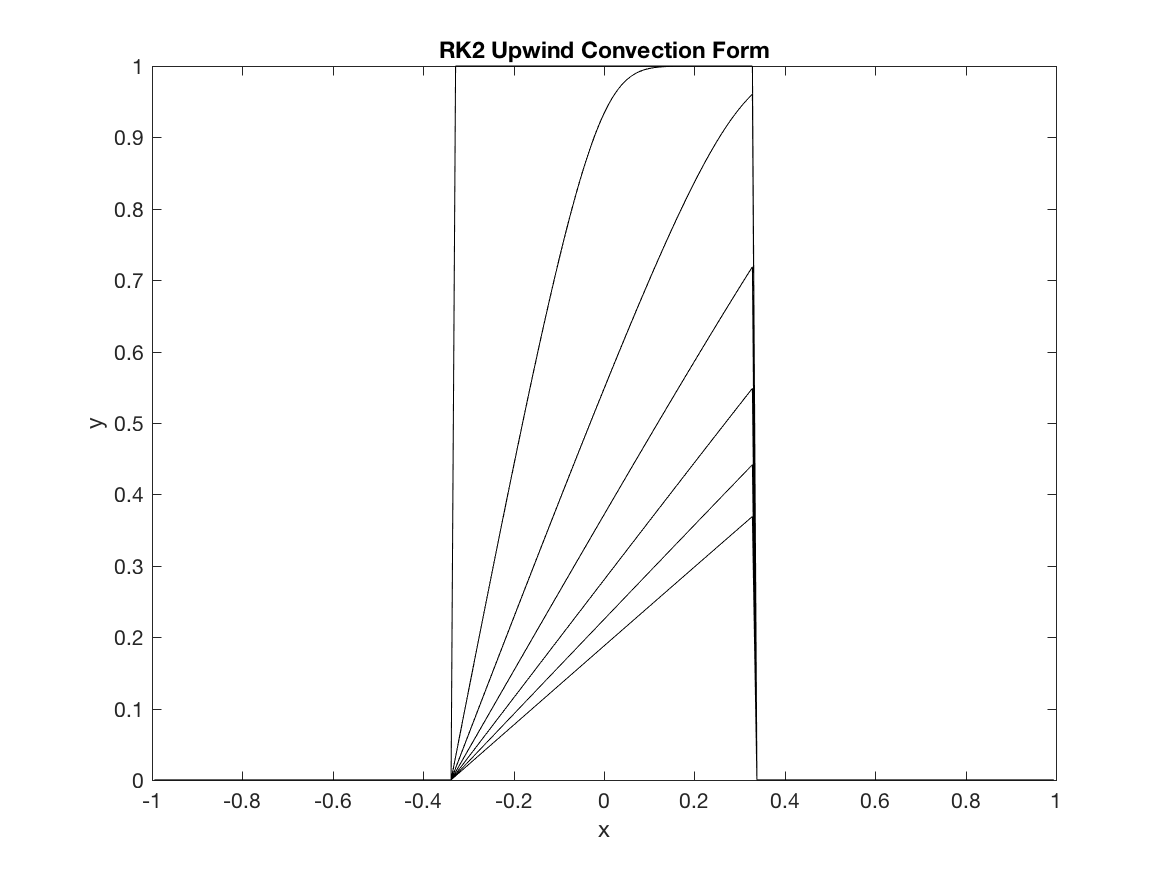
\includegraphics[scale=0.5]{Figures/08_14.png}
    \end{center}
    The Lax-Wendroff method propogates the shock at the correct speed, but it
    does not properly find the rarefaction/expansion.
    Also the Lax-Wendroff has spurious oscillations around the shocks.
    \begin{center}
      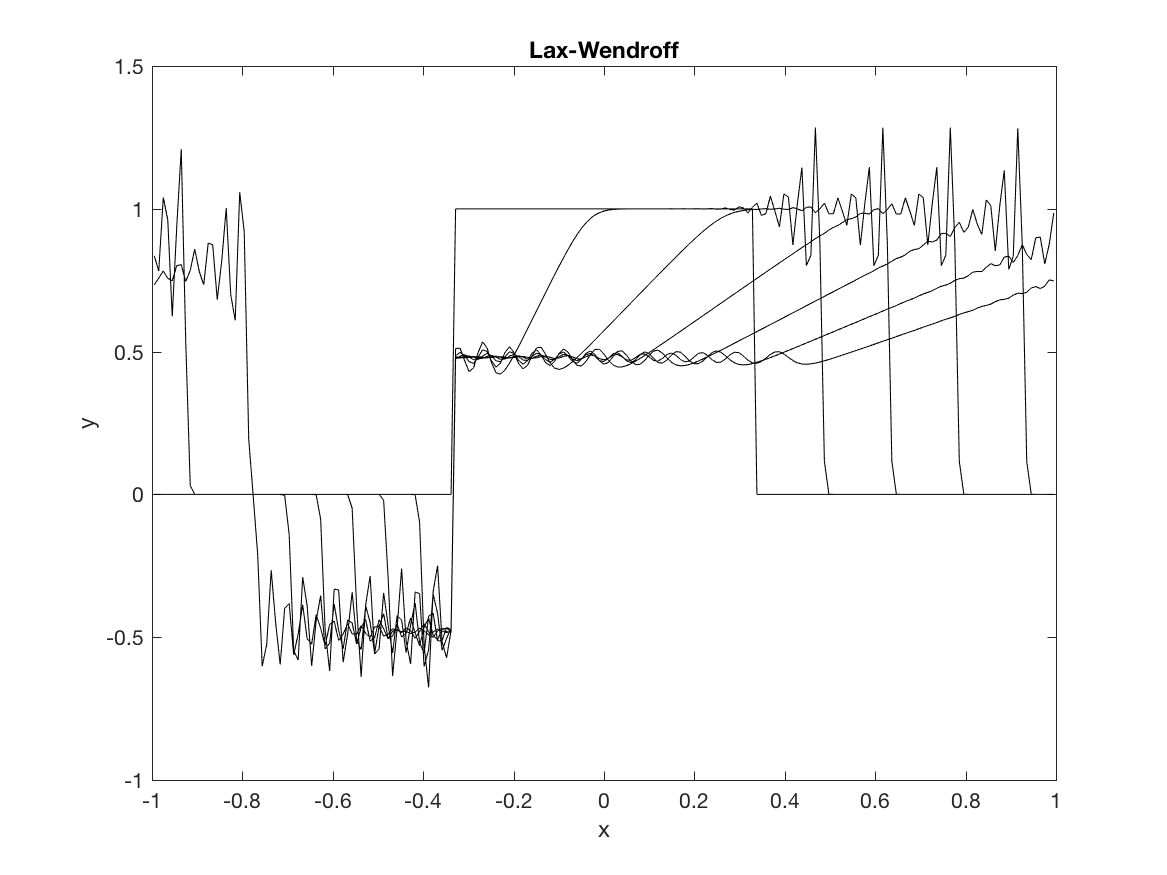
\includegraphics[scale=0.5]{Figures/08_15.png}
    \end{center}

\end{enumerate}
\end{document}
